\providecommand{\main}{..}
\documentclass[\main/master.tex]{subfiles}
\begin{document}
\chapter{thesis aims}\label{chp:example-2}
\section{Measurement Method}
\subsection{Measurement Method}
\subsubsection{Measurement Method}
The Cavendish experiment, is constructed using a torsional pendulum with a front mirror. The angle displaement is causing a mirror tilt. Optical measurement of angle displaement is made with a split detector using interferometric technique. 
\par
Shot noise using a split detector in an interferometric technique is even on all frequencies. Shot limit when integrating over a long time.
\begin{equation}
\Delta\theta = \frac{1}{4\sqrt{2}\pi}\frac{\lambda}{L\sqrt{N}} \approx
4\cdot10^{-14} [\frac{rad}{Hz}]    \label{eqn:gravitation_tourqe}
\end{equation}
When the gravitational force is measured using a torsional pendulum, there are noise limitation to the measuremnt sensetivity. The limitation are higher than the shot noise limit, meaning that reducing the noise could achieve higher sensetivity. The noises on the pendulum are unknown magnetic noise, acoustic waves and random fluctuations due to thermal brownian motion.Friction is also limiting the pendulum response. 
\par
Pendulum is placed inside vacuum reducing brownian motion, acoustic waves and friction, vacuum chamber is reducing magnetic noise by faraday cage. At vacuum the brownian motion from envirement coupling is reduced, but still is the main noise source. The system quantum uncertainty at a specific temperature due to brownian motion (assuming noise is much higher than basic energy level). 
\begin{equation}
\frac{1}{2}\kappa (\delta\theta_{max})^2= \frac{1}{2}KT  \label{eqn:radiation force}
\end{equation}
\begin{equation}
\delta\theta_{max} = \sqrt{\frac{KT}{\kappa}}\propto{T}  \label{eqn:radiation force}
\end{equation}

The noise reductance enables to damp and cool the pendulum temperture. Damping is made using a PID feedback loop. The feedback damping can dynamically damp the noises, without pre-knowledge of the existing noises. PID would reduce all noises, and reduce the temperature. Having an effective lower temperature would enable measuring smaller angles enlarging the SNR and the measuremnt sensetivity.
\par
When PID tuned correct damped pendulum is at critical damping and ossiclations become smaller. PID error is getting samller and damping response becomes small. 
\begin{equation}
e(t) = \delta\theta(t)   \label{eqn:pid_error}
\end{equation}
\begin{equation}
u(t) = K_Pe(t)+K_I\int_{0}^{t}e(t)+K_D\frac{de(t)}{dt}   \label{eqn:PID_eq}
\end{equation}

Introducing a new mass adds a constant new tourqe to the system, which the PID is compensating with a propotional gain $K_P$. The PID response becomes mainly an inverse tourqe. Assuming the mass is moving at low frequencies, when integrating over short periods the angle is constant in time.
\begin{equation}
e(t) = \delta\theta(t) + \theta_g    \label{eqn:PID_measurement}
\end{equation}
\begin{equation}
u(t) = u[ \delta\theta(t)] + K_P\theta_g(t) \label{eqn:PID_measurement_eq}
\end{equation}
\begin{equation}
U = \int u(t)dt  \approx K_P\theta_g\Delta t \label{eqn:PID_measurement_eq}
\end{equation}
\begin{equation}
\tau(r) = L\frac{GmM}{r^2} =  \kappa\theta_g = \kappa\frac{U}{K_P\Delta t}      \label{eqn:pid_gravitation_tourqe}
\end{equation}
\begin{equation}
\kappa =\frac{8\pi^2ml^2}{T^2}    \label{eqn:empirical_tourqe}
\end{equation}

The measurement of that response is fast and accurate. The measurement sytem is measuring with fast response (short integration time) and high accuracy low frequency garvity fields. 

 
 
 
 





\section{accuracy}
\doublespacing
\hspace{5 mm} This another example chapter with a working reference as see in Chapter~\ref{chp:example-1}. There I also made an example of an equation, see Eqn.~\ref{eqn:energy-mass-equivalence-relation}. We also created an example image, see Fig.~\ref{fig:sine-wave}.
\begin{figure}[htbp]
	\centering
	\fbox{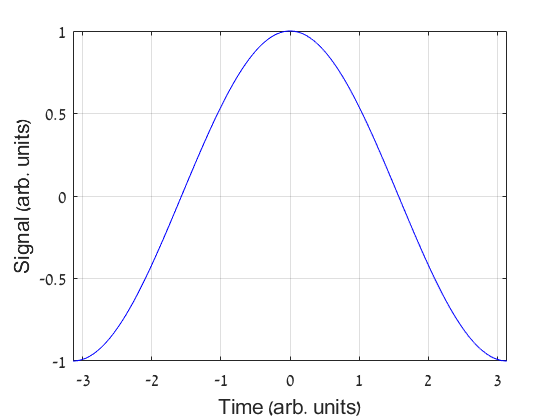
\includegraphics[scale=0.75]{\main/images/chapter_2_example/img_example_2.png}}
	\caption[Another Example Image]{Another Example Image. This image is also labeled internally so we can referenc it throughout the text.}
	\label{fig:cosine-wave}
\end{figure}
\end{document}